\section{Lezione 19}%
\label{sub:Lezione 19}
\subsection{Mappa di Henon}%
\label{sub:Mappa di Henon}
La mappa di Henon è stata al centro di numerose ricerche sui sistemi caotici e non lineari. Henon ebbe l'idea di modellizzare con questa mappa il moto degli oggetti celesti. Secondo il suo modello, per determinati parametri iniziali, il moto sfocia nel caos.\\
Costruiamo la mappa in due step, un primo step è un "twist" con un termine $-x^2$, chiamiamo questa trasformazione $T_1$:
\[
    T_1: \quad
    \begin{cases}
        x' = x_i\\
	y' = y_i-x_i^2
    \end{cases}
.\] 
Mentre il secondo step ($T_2$) è una rotazione del primo:
\[
    T_2: \quad
    \begin{pmatrix} x_{i+1} \\ y_{i+1} \end{pmatrix} =
    \begin{pmatrix} 
	\cos\alpha  &  - \sin\alpha  \\
	\sin\alpha  &  \cos\alpha
    \end{pmatrix} 
    \begin{pmatrix} x' \\ y' \end{pmatrix} 
.\] 
In conclusione abbiamo $T = T_1\cdot T_2$:
\[
    \begin{cases}
	x_{i+1} = x_i\cos\alpha-(y_i-x_i^2)\sin\alpha\\
	y_{i+1} = x_i\sin\alpha + (y_i-x_i^2)\cos\alpha
    \end{cases}
.\] 
\begin{figure}[H]
    \centering
    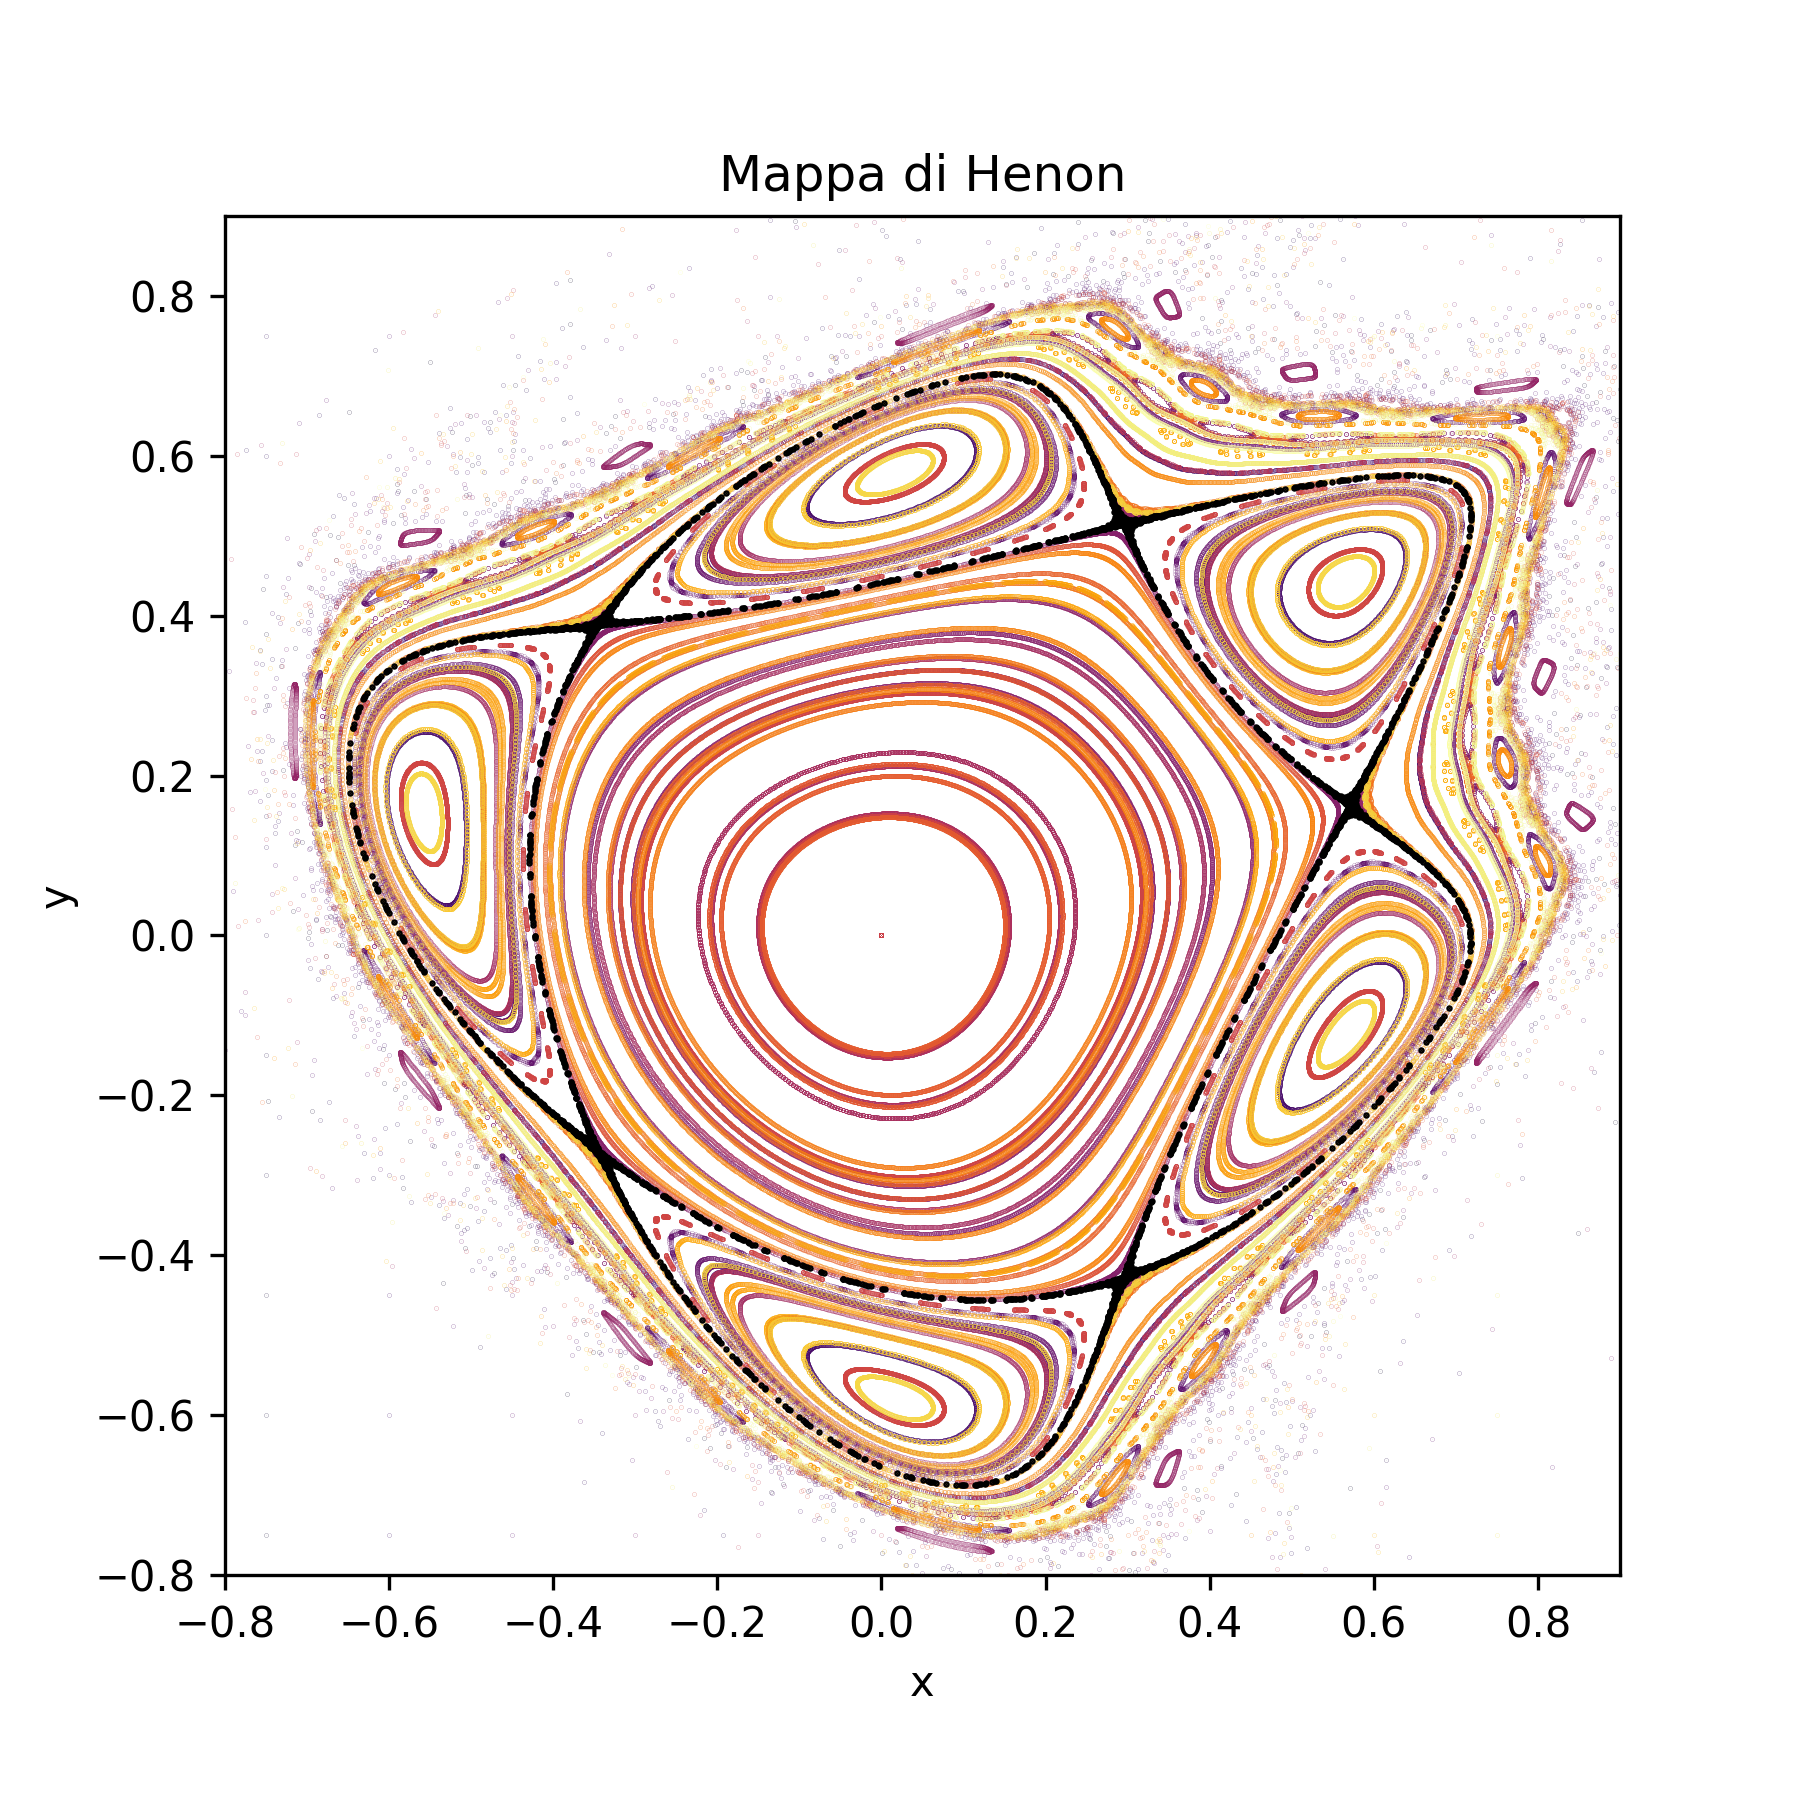
\includegraphics[width=0.5\textwidth]{figures/18_Henon_map.png}
    \caption{\scriptsize Mappa di Henon al variare dei parametri iniziali di $x$ e $y$ con $\alpha = 1.328$. Si è messa enfasi sulla traiettoria passante per il punto fisso (in nero). Notiamo come le traiettorie esterne sfocino già nel caos. Realizzata in Fortran e Python.\\
    In questa immagine c'è molto di più di quel che si vede, provando a valutare il moto negli intorni dei punti fissi appaiono strutture di vario genere, piccoli tori circondati da caos (provare a giocare con le condizioni iniziali per vedere).}
    \label{fig:figures-18_Henon_map-png}
\end{figure}
\noindent
Possiamo chiederci se questa mappa sia Area preserving. \\
Per quanto riguarda la rotazione $T_2$ non ci sono problemi, sappiamo che ogni rotazione ha un Jacobiano unitario. \\
La mappa $T_1$ invece (usiamo la notazione di sopra con $x', y'$):
\[
    \frac{\partial x'}{\partial x_i} = 1 \qquad \frac{\partial x'}{\partial y_{i}} = 0
\] 
\[
    \frac{\partial y'}{\partial x_i} = 0  \qquad  \frac{\partial y'}{\partial y_{i}} = 1
.\] 
Quindi abbiamo che il determinante della matrice delle derivate miste è unitario anche per $T_1$, di conseguenza la trasformazione è Area preserving e potrebbe essere attribuita ad una qualche Hamiltoniana. Quale Hamiltoniana genera questa mappa?
\subsection{Legare una mappa ad una Hamiltoniana}%
\label{sub:Legare una mappa ad una Hamiltoniana}
Prendiamo una Hamiltoniana del tipo:
\begin{equation}
    H(\vect{q}, \vect{p})=\sum_{}^{} \frac{1}{2}p_i^2 + V(\vect{q})
    \label{eq:19_H}
\end{equation}
\paragraph{L'integrazione di Eulero non è Area preserving}%
\label{par:Integrazione di Eulero}
Possiamo provare a discretizzare le equazioni del moto in questo modo:
\[
    \begin{cases}
        q_{i+1}=q_i + hp_i\\
	p_{i+1}=p_i - h \frac{\partial V}{\partial q_i} 
    \end{cases}
    \qquad
    h = \Delta t
.\] 
Possiamo scrivere la mappa in forma di matrice (in questo modo si isola lo Jacobiano):
\[
    \begin{pmatrix} q_{i+1}\\ p_{i+1} \end{pmatrix} =
    \begin{pmatrix} 
	1      & h \\
	- hV'' & 1
    \end{pmatrix} 
    \begin{pmatrix} q_i \\p_i \end{pmatrix}
.\] 
Dove la derivata seconda $V''$ appare perché si scrive:
\[
    \frac{\partial V}{\partial q_i} = \frac{\partial ^2V}{\partial q_i^2} \partial q_i
.\] 
Per rendere proporzionale a $q$ il termine con la derivata parziale di $V$. \\
Il determinante della trasformazione non è unitario:
\[
    \text{det} = 1 + h^2V'' \neq 1
.\] 
Quindi la mappa che si ottiene da una integrazione con Eulero non è area preserving. Integrando con questo metodo l'Hamiltoniana perderemo molto rapidamente le caratteristiche del nostro sistema fisico.
\paragraph{Eulero "a due step" è Area preserving}%
\label{par:Eulero "a due step" è Area preserving}
Prendiamo la seguente variante dell'integrazione con Eulero:
\[
    \begin{cases}
        q_{i+1}=q_i + hp_i\\
	p_{i+1}=p_i - h V_{i+1}
    \end{cases}
.\] 
In cui il termine $V'_{i+1}$ è la derivata del potenziale rispetto a $q_{i+1}$. \\
Così facendo il termine in basso a sinistra nello Jacobiano descritto sopra non c'è:
\[
    J = 
    \begin{pmatrix} 
	1 & h\\
	0 & 1
    \end{pmatrix} 
.\] 
Ed il determinante di questa matrice è 1: abbiamo una integrazione AP (Area preserving).\\
Il problema è che, a differenza delle equazioni agli incrementi di Eulero, questa integrazione non deriva direttamente dalle equazioni di Hamilton discretezzate dell'Hamiltoniana \ref{eq:19_H}. Da quale Hamiltoniana derivano?\\
Si può dimostrare che questa H deve esser della forma:
\begin{equation}
    H = \frac{p^2}{2} + h V(q)\delta(t-ih) \qquad i \in \mathbb{N}
    \label{eq:19_H_poincare}
\end{equation}
Per un tempo $h'$ abbiamo una equazione per particella libera ($H=p^2 /2$), tale Hamiltoniana si sa integrare (equazioni del moto lineari).
\[\begin{aligned}
    & q_{i+1}=q_i + hp_i\\
    & p_{i+1}=p_i
.\end{aligned}\]
Quindi lontano dalle $\delta$ abbiamo una specie di twist map.
Ai tempi $t=ih$ il nostro oggetto prende un colpo dal potenziale.\\
Immaginiamo di iniziare l'integrazione in un tempo tra $\left[ih, (i+1)h\right]$, in tal caso si ha per $q$ l'equazione scritta sopra, mentre per $p$ abbiamo una sorpresa:
\[
    \dot{p} = - \frac{\partial V}{\partial q}
.\] 
Se la integriamo nel tempo sopravvivono soltanto dei pezzi negli intorni di $(i+1)h$ (il tempo $ih$ è già passato):
\[
    p_{i+1} - p_i = -\int\limits_{(i+1)h-\epsilon}^{(i+1)h+\epsilon} V' dt  = - h V_{i+1}'
.\] 
Notiamo che si potrebbe anche invertire il ruolo di $p$ e $q$, effettuando prima il "calcio" e successivamente l'evoluzione:
\[\begin{aligned}
    & q_{i+1} = q_i + p_{i+1}h\\
    & p_{i+1} = p_i - V_i'h
.\end{aligned}\]
\paragraph{Analogia con le mappe di Poincare}%
\label{par:Analogia con le mappe di Poincare}
La questione del passaggio dall'Hamiltoninana di partenza ad una mappa (e viceversa) è quindi risolta? Cosa significa fisicamente risolvere per una Hamiltoniana come quella di equazione \ref{eq:19_H_poincare}?\\
Sorprendentemente signfica che stiamo studiando una mappa di Poincare: fissare degli istanti di "osservazione" del sistema con la $\delta$ significare fissare dei piani a tempi fissi nello spazio ($q,p,t$), esattamente quello che si fa con una mappa di Poincare.\\
Infatti fissare un piano di osservazione
\footnote{ad esempio $y=0$ come nell'esempio della lezione scorsa}
significa aspettare gli istanti in cui l'oggetto passerà nuovamente da tale piano, quindi è esattamente l'analogo di quello che stiamo facendo adesso.
\subsection{Introduzione alla mappa standard}%
\label{sub:Introduzione alla mappa standard}
La maggior parte degli studi sul caos è stato effettuato sulla mappa standard. Tale mappa ha la seguente struttura:
\begin{redbox}{Mappa standard}
 \[\begin{aligned}
    & q_{i+1} = q_i + p_{i+1}\\
    & p_{i+1} = p_i + \frac{k}{2\pi}\sin (2\pi q_i)
.\end{aligned}\]   
\end{redbox}
\noindent
In cui si sceglie mod($q$)=mod($p$)=1
\footnote{Su wikipedia si dice che solitamente $p, q$ sono presi modulo $2\pi$ (perché non si divide per $2\pi$ l'incremento con $k$), quindi si divide $p$ e $q$ per $2\pi$ ogni step e se ne prende il resto.Nel caso di modulo 1 il resto è il numero stesso.}
.\\
Notiamo anche che il potenziale in questione è quello di un pendolo.
\begin{figure}[H]
    \centering
    \includegraphics[width=0.5\textwidth]{figures/19_standard_map.png}
    \caption{\scriptsize Mappa standard integrata con $k=0.97$. Si nota la presenza di strutture che ricordano tori invarianti, in altre zone è invece evidente la presenza di caos.}
    \label{fig:figures-19_standard_map-png}
\end{figure}
\noindent
Questa mappa è sicuramente Hamiltoniana, infatti si ha uno Jacobiano:
\[
     M = 
     \begin{pmatrix}
	 1 & 0 \\
	 k \cos(2\pi q_i) & 1
     \end{pmatrix} 
.\] 
Abbiamo un termine non lineare in basso a sinistra, tuttavia ai fini del determinante questo non ha importanza.
\subsection{Studio dei punti fissi per un mappa Hamiltoninana}%
\label{sub:Studio dei punti fissi per un mappa Hamiltoninana}
Definiamo la mappa come la trasformazione $T$, cerchiamo di capire cosa avviene nella mappa nei punti $x^*$ tali per cui:
\[
    x^* = T(x^*)
.\] 
In particolare ci concentriamo su un intorno di questi cercando di linearizzare il problema:
\[
    \vect{x} = \vect{x}^* + \delta\vect{x}
.\] 
\[\begin{aligned}
    \implies  & \vect{x}_{n+1} = \vect{x}^* + \delta\vect{x}_{n+1} = T(\vect{x}^* + \delta\vect{x}_n) = \\
	      & \simeq T(\vect{x}^*) + \left.\frac{\partial T}{\partial \vect{x}} \right|_{\vect{x}^*}\delta\vect{x}_n
.\end{aligned}\]
Abbiamo quindi che il comportamento al punto fisso è determinato dalla matrice delle derivate miste:
\[
    \delta\vect{x}_{n+1} = \left.\frac{\partial T}{\partial \vect{x}} \right|_{\vect{x}^*}\delta\vect{x}_n \delta\vect{x}_n
.\] 
Esplicitamente:
\[
    \begin{pmatrix} \delta x_{n+1} \\ \\ \delta y_{n+1} \end{pmatrix} = 
    \begin{pmatrix} 
	\frac{\partial T_x}{\partial x} && \frac{\partial T_x}{\partial y} \\
					&&\\
	\frac{\partial T_y}{\partial y} && \frac{\partial T_y}{\partial y} 
    \end{pmatrix} 
    \begin{pmatrix} \delta x_{n} \\ \\ \delta y_{n} \end{pmatrix} 
.\] 
Essendo la mappa per ipotesi Hamiltoninana si ha che matrice al centro (che chiamiamo $M$) ha determinante unitario, gli autovalori di questa matrice possono essere ricavati tramite l'equazione secolare:
\[\begin{aligned}
    \text{det}(M-\lambda\mathbb{I})=&\lambda^2-\lambda\text{tr}(M)+\text{det}(M) = \\
    =&\lambda^2-\lambda\text{tr}(M)+1
.\end{aligned}\]
\[
    \lambda_{\pm} = \frac{\text{tr}(M)\pm\sqrt{(\text{tr}(M))^2-4}}{2}
.\] 
ci sono allora due possibilità per gli autovalori:
\begin{itemize}
    \item $\left|\text{tr}(M)\right|<2$: autovalori complessi coniugati.
    \item $\left|\text{tr}(M)\right|>2$: autovalori reali.
\end{itemize}
Il fatto che il determinante di $M$ sia unitario comporta anche che il prodotto tra i due autovalori faccia 1:
\[
    \lambda_+\cdot \lambda_- = 1
.\] 
Quindi possiamo definire $\lambda_+ = \lambda$, di conseguenza:
\[
    \lambda_+ = \lambda  \qquad \lambda_- = \frac{1}{\lambda}
.\] 
\paragraph{Autovalori reali}%
\label{par:Autovalori reali}
Consideriamo il caso in cui gli autovalori sono reali con autovettori corrispondenti $\vect{\omega}$, l'evoluzione di questi vettori avrà la seguente forma per definizione:
\[
    \delta\vect{\omega}_{n+1} = 
    \begin{pmatrix} 
	\lambda  & 0 \\
	0 & 1 /\lambda
    \end{pmatrix} 
    \delta\vect{\omega}_n
.\] 
Quindi l'evoluzione degli autovettori si distingue in due casi:
\begin{enumerate}
    \item $\lambda > 0$:
	Allora abbiamo le due evoluzioni per gli autovettori:
	\[
	    \omega^{(+)}_n = \lambda^n \omega_0; \qquad \omega^{(-)}_n = \left(\frac{1}{\lambda}\right)^n \omega_0
	.\] 
	Quindi in una direzione abbiamo una espansione, nell'altra una contrazione.
    \item $\lambda < 0$: In questo caso si ha l'analogo del caso precedente però ad ogni step gli assi invertono la loro direzione
	\[
	    \omega^{(+)}_n = (-1)^n\lambda^n \omega_0; \qquad \omega^{(-)}_n = (-1)^n\left(\frac{1}{\lambda}\right)^n \omega_0
	.\] 
\end{enumerate}
Nel caso (1) possiamo anche dire qualcosa in più sul nostro sistema: scriviamo l'equazione di $\omega_n$ in termini di esponenziali
\[
    \omega_n = \omega_0 \exp (n\ln\lambda)
.\] 
In questa equazione il termine $n$ gioca il ruolo di un tempo, in questo modo si scopre che la scala di evoluzione del sistema $\tau$ è:
\[
    \tau\sim \frac{1}{\ln\lambda}
.\] 
Questa è la scala con la quale gli oggetti si allontanano/collassano su un punto fisso.\\
Questo studio dei punti fissi ci serve per capire cosa succede in un sistema quando si rompe il teorema KAM.
\subsection{Caos e rottura del teorema KAM}%
\label{sub:Caos e rottura del teorema KAM}
Prendiamo la seguente mappa in coordinate azione angolo:
\[\begin{aligned}
    & \varphi_{n+1} = \varphi_n + \frac{\partial }{\partial I_{n+1}} S_0(I_{n+1})\\
    & I_{n+1} = I_n
.\end{aligned}\]
Questa è molto simile ad una Twist map. A destra della prima equazione abbiamo il termine $\partial_{I_{n+1}}S_0$, questo può essere associato al rapporto tra le frequenze della Hamiltoniana predetto in generale per le twist map nella lezione precedente.
\[
    \partial_{I_{n+1}}S_0 \sim 2\pi  \frac{\omega_1}{\omega_2}
.\] 
Nel seguito supponiamo che il termine $\alpha(I) = \omega_1 /\omega_2(I)$ proporzionale a $I$, quindi abbiamo una specie di twist map come nella seconda figura di Figura \ref{fig:-figures-18_twist_tetha_r-png}.\\
Il teorema KAM ci assicura che i primi tori che si rompono sono quelli per il quale il rapporto $\omega_1 /\omega_2$ è un numero razionale. \\
Prendiamo una situazione in cui alcuni tori previsti dal teorema KAM sono preservati mentre si rompe un singolo toro di quelli razionali, cerchiamo di capire cosa si vede nello spazio delle fasi in questo caso.
L'idea per far questo è sempre quella di scrivere una teoria perturbativa su $S$:
\[\begin{aligned}
     & \varphi_{n+1} = \varphi_n + \frac{\partial }{\partial I_{n+1}} S_0 + \epsilon\frac{\partial }{\partial I_{n+1}} S_1(I_{n+1}, \varphi_n)\\
     & I_{n+1} = I_n + \epsilon\frac{\partial }{\partial \phi_{n}} S_1(I_{n+1}, \varphi_n) 
.\end{aligned}\]
Come sappiamo sono i termini perturbativi introdotti in queste equazioni a rompere il toro. Possiamo vedere cosa avviene alle curve che si rompono.\\
Partiamo dai tori imperturbati, questi nello spazio $I, \varphi$ faranno delle circonferenze poiché $I$ si conserva. \\
Prendiamo allora 3 di questi tori aventi $I$ crescente (che chiamiamo $C_+, C, C_-$), questi formeranno 3 circonferenze concentriche come in figura \ref{fig:19_tori}. \\
Scegliamo il toro centrale $C$ tale che la sua frequenza sia razionale, quindi ci aspettiamo che sia un toro che si rompe prima degli altri due limitrofi.\\
Si effettua un cambio di sistema di riferimento in modo tale da rendere i punti del toro centrale fermi, gli altri due tori avranno la caratteristica (nel nuovo sistema) di ruotare uno in senso orario e l'altro in senso antiorario poiché $\omega\propto I$.
\begin{figure}[H]
    \centering
    \incfig{19_tori}
    \caption{\scriptsize Cambio di sistema di riferimento, i punti del toro al centro sono fermi poiché siamo in un sistema rotante con la $\omega$ di quel toro. \\
    Il toro più grande aveva una $\omega$ più grande, il toro più piccolo invece una $\omega$ più piccola rispetto al centrale. Per questo motivo il primo gira in senso orario ed il secondo in senso antiorario dopo la trasformazione.}
    \label{fig:19_tori}
\end{figure}
\noindent
A questo punto possiamo accendere la perturbazione (si reinserisce nelle equazioni i termini con $\epsilon$). In questo modo i nuovi tori $C_{-,\epsilon}$, $C_{+, \epsilon}$ subiscono una piccola perturbazione rispetto alle loro posizioni iniziali, il toro centrale $C$ invece si rompe e cessa di esistere.
\begin{figure}[H]
    \centering
    \incfig{19_tori_rotto}
    \caption{\scriptsize Il toro $C$ si rompe in seguito alla accensione della perturbazione, ciò che resta di lui è l'alone nero al centro a rappresentare il caos (in realtà stiamo cercando di scoprire cosa succederà ai punti al centro, quindi nel proseguo immagineremo soltanto che quel toro non esiste più e dobbiamo valutare dove vanno a finire i punti). In magenta abbiamo la varietà di punti fermi tra i due tori che deve esistere necessariamente per la continuità di $\varphi$ ed $I$.}
    \label{fig:19_tori_rotto}
\end{figure}
\noindent
Dopo la rottura del toro $C$  tra i due tori dovrà necessariamente esistere una varietà di punti aventi $\omega =0$. Questo perché il toro esterno ed il toro interno hanno $\omega$  di segno opposto in questo sistema, tracciando una linea che passa per i due tori necessariamente deve esistere un punto in mezzo che annulla la $\omega$. \\
Chiamando la mappa $T_{\epsilon}$ abbiamo che, per i punti appartenenti alla varietà rimasta fissa:
\[
    \varphi^* = T_{\epsilon}(\varphi^*)
.\] 
Sicuramente la varietà rossa dei punti fermi non è invariante, quindi evolverà negli step successivi. L'unico modo per cui può evolvere questa varietà è quello di variare la componente radiale poiché quella angolare è fissata per definizione di questa curva. \\
La cosa importante è che i punti fissi dovranno appartenere per ogni step a tale varietà, per tali punti deve valere sempre:
\[
    I^* = T_{\epsilon}(I^*)
.\] 
\begin{figure}[H]
    \centering
    \incfig{19_tori_step}
    \caption{\scriptsize Andamento della varietà con i punti aventi $\omega =0$ al variare degli step della mappa, nella prima figura in alto a sinistra si mostra la mappa imperturbata, in tal caso la varietà dei punti fermi corrisponde con il toro invariante per costruzione.\\
    Le due figure successive corrispondono all'aver acceso la perturbazione, le curve magenta e blu pertanto non sono tori poiché in questa zona c'è il caos. In nero sono presenti i punti fissi.}
    \label{fig:19_tori_step}
\end{figure}
\noindent
La cosa interessante da capire è la struttura dei punti fissi, questa ci dirà in che modo i tori si stanno spaccando. \\
Guardiamo da vicino una zona della figura precedente: 
\begin{figure}[H]
    \centering
    \incfig{19_tori_ingrandimento}
    \caption{\scriptsize Ingrandimento su zona con punti fissi, le frecce indicano la direzione di variazione della varietà fissa o isocrona.}
    \label{fig:19_tori_ingrandimento}
\end{figure}
\noindent
Possiamo vedere che tra la varietà del primo step e quella del secondo i punti devono necessariamente avvicinarsi/allontanarsi dal punto fisso. Questo è dovuto al fatto che $\omega \propto I$, quindi per passare da zone con $I$ maggiore/minore c'è bisogno di accelerare/rallentare.\\
Questa particolarità ci dice che i punti fissi sono un alternanza di punti iperbolici ed ellittici. Tutti questi punti fissi vivono tra i due tori quasi conservati $C_{\pm, \epsilon}$.\\
Prendiamo in considerazione il punto iperbolico in figura (quello in basso) e cerchiamo di capire cosa viene in un suo intorno.\\
Sappiamo che un punto iperbolico è caratterizzato da due curve instabili (che si allontanano esponenzialmente dal punto) e da due curve stabili (che cadono esponenzialmente nel punto), tali curve vengono chiamate Manifold.
\begin{figure}[H]
    \centering
    \incfig{19_stab_instab}
    \caption{\scriptsize Curve stabili ed instabili per il punto iperbolico. Notiamo che non devono necessariamente coincidere con le curve isocrone, l'importante è che siano consistenti con le direzioni di figura \ref{fig:19_tori_ingrandimento}.\\
    Dobbiamo anche precisare che le curve colorate siano delle varietà stabili mentre le linee con le frecce sono delle possibili mappe di Poincare.}
    \label{fig:19_stab_instab}
\end{figure}
\noindent
Può succedere che le due curve nere, nelle vicinanze del punto fisso, si incrocino in un punto (diverso dal punto iperbolico). L'intersezione è quasi inevitabile visto che il punto iperbolico è schiacciato tra due tori: i manifold (curve nere) sono costretti a "piegarsi" prima o poi per non oltrepassare il toro.
\begin{figure}[H]
    \centering
    \incfig{19_intersezione}
    \caption{\scriptsize Intersezione dei Manifold nei pressi di un punto fisso.}
    \label{fig:19_intersezione}
\end{figure}
\noindent
Immaginiamo adesso di far evolvere le traiettorie nella direzione del punto di incrocio del manifold. Iterando la mappa si avrà una situazione del tipo:
\begin{figure}[H]
    \centering
    \incfig{19_itero_fisso}
    \caption{\scriptsize Iterazioni della mappa per punti attorno al punto di incrocio dei manifold.}
    \label{fig:19_itero_fisso}
\end{figure}
\noindent
Adesso se si prova ad iterare la mappa per il punto $P$  si ottiene un paradosso: l'iterazione $T(P)$  dovrebbe stare davanti sia a $T(x)$  che a $T(x')$.
L'unica situazione possibile è che i manifold si incrocino ancora in un punto $T(P)$.
\begin{figure}[H]
    \centering
    \incfig{19_manifold_incrocio1}
    \caption{\scriptsize Iterazione della mappa nei pressi del punto di intersezione dei manifold: si genera un ulteriore punto di intersezione dei manifold.}
    \label{fig:19_manifold_incrocio1}
\end{figure}
\noindent
Abbiamo quindi generato una zona chiusa tra le intersezioni dei manifold di area $A$.
Per una iterazione successiva il punto $T(P)$ dovrà andare in un punto $T^2(P)$ che è ancora un altra intersezione di manifold, quindi le due curve nere si intersecheranno ancora, generando un altra superficie separata di area $A$ (la stessa di prima perché la mappa è area preserving).\\
Adesso dobbiamo ricordare che i manifold si allontanano/avvicinano esponenzialmente al punto fisso. Possiamo notare nella figura \ref{fig:19_manifold_incrocio1} che al momento della prima iterata della mappa (quando creo $T(P)$) il manifold uscente ha fatto più strada del manifold entrante.\\
Tenendo di conto di questo nelle iterate successive lo spostamento dal punto $T(P)$ per il punto $T^2(P)$ sarà maggiore nella direzione di allontanamento dal punto fisso rispetto a quella di avvicinamento.\\
Come conseguenza oltre a preservare l'area le curve generate saranno sempre più allungate e schiacciate come in figura %\ref{}
\begin{figure}[H]
    \centering
    \incfig{19_itero2}
    \caption{\scriptsize Seconda iterazione della mappa: si genera un secondo punto di intersezione. \\ Notiamo come la seconda "area" generata sia stata rappresentata piegata, questo perché i manifold sono linee separatrici dello spazio delle fasi: non si possono attraversare.}
    \label{fig:19_itero2}
\end{figure}
\noindent
Iterando la procedura ancora e ancora nello spazio delle fasi succederà un gran casino, i manifold oscilleranno su loro stessi generando altre intersezioni dal quale potrebbero nascere altre oscillazioni\ldots è caos.\\
Queste strutture oscillanti possono generarsi da uno stesso punto fisso (\textbf{strutture omocliniche}) oppure a partire dalla intersezione di manifold provenienti da punti fissi diversi (\textbf{strutture eterocliniche}).
Nota fenomenologica: Le zone eterocliniche si formano dagli incroci di varietà degli altri punti, quindi per vedere queste varietà eterocliniche c'è bisogno di avere un sistema già "abbastanza" caotico. 
\subsubsection{Strutture autosimilari nei punti ellittici}%
\label{subsub:Strutture autosimilari nei punti ellittici}
Nei pressi dei punti ellittici invece abbiamo delle isole invarianti, infatti all'interno di queste strutture non può penetrare il caos generatosi attorno ai punti iperbolici circostanti. \\
In pratica si ha che "ingrandendo" la zona di un punto ellittico si osserva una struttura del tutto analoga a quella originale: anche all'interno dell'isola invariante ci saranno punti fissi iperbolici ed ellittici a formare quindi una struttura self similare.
\clearpage
